% Chapter Template

\chapter{MECOM 2012} % Main chapter title

\label{C3} % Change X to a consecutive number; for referencing this chapter elsewhere, use \ref{ChapterX}

\lhead{Capítulo 3. \emph{MECOM 2012}} % Change X to a consecutive number; this is for the header on each page - perhaps a shortened title

%----------------------------------------------------------------------------------------
%	SECTION 1
%----------------------------------------------------------------------------------------
\section{Abstract}

Amorphous metals, i.e. without defined crystal structure; are increasingly used in modern life, showing great potential as advanced engineering materials, due to some of its characteristic properties such as high hardness and moldability, high resilience, high mechanical strength and high wear resistance, among others. All these properties allow obtaining parts with complex shapes and high strength, which increases their chances for industrial application. However, many details of the mechanical behavior are still unknown, and the currently used models and theories are far from predictive.
One of the possibilities to determine constitutive parameters, and thus study the response of these materials, is by using atomistic calculations. In this paper we present results obtained with molecular dynamics (MD) simulations, of an amorphous metal (CuZr). In particular, constitutive parameters such as elasticity modulus, are determined for samples at different temperatures and subjected to both tension and compression. The results obtained are relevant for understanding the mechanical behavior of the material, such as stress-strain and temperature-strain relationships. Additionally, it is possible to observe, under uniaxial tension, the nucleation and growth of a void due to high stress and strain rate values.

\section{INTRODUCTION}
Solid materials without an ordered structure, i.e. amorphous, are generally called "glasses". Particular cases of great scientific and technological interest are metallic glasses, which are metallic alloys with mechanical properties that outperform the most common crystalline alloys (Luborsky, 1983; Greer, 1995). It is known that metals easily form crystals when cooled (Callister, 1995; Smith, 1996). However, using a sufficiently fast cooling rate and controlling the composition of the alloy it is possible to obtain amorphous structures (Liebermann, 1993), with the elasticity of polymers and the resistance of metals (Telford, 2004), also having high strength and moldability. All these properties enable the creation of parts with complex shapes and high resistance, which further increases their chances of industrial applications. Thanks to the above properties, these materials have received great interest as structural materials in recent years (Chen, 1974; Lowhaphandu et. al, 1999; Inoue, 2000, Wang et al., 2004, Ashby et al., 2006, Zhang et. al, 2007; Schuh et. al, 2007), including, for example, amorphous structural steels (Lu et al., 2004), biomedical materials (Zberg, 2009) or even aerospace materials (Peker, 1993), to name a few.

Metallic glasses can generally be classified as conventional metallic glasses or bulk metallic glasses (BMG) (Wang et al., 2004, Miller et al., 2007). BMG have recently been employed as matrix phase in composite materials, thus improving the various original properties of the dispersed phase such as mechanical, magnetic properties, etc. (Telford, 2004; Lu, 2011). In the particular case of metallic glasses under plastic strain, with the appearance of shear bands, it is customary to address the problem through a focus on nanoscale behavior (Ogata, 2006, Guan, 2010), or through an approach using continuum mechanics (Malvern, 1969).

Molecular dynamics (MD) simulations are often used to study nanoscale properties (Allen and Tildesley, 1987). MD simulations are a very powerful technique that allows solving, using classical mechanics, problems with many bodies, given an interaction between atoms. One advantage of MD is that strain, stress, temperature, speed, etc. are all known in detail (Allen and Tildesley, 1987). From this information large number of phenomena can be studied, such as phase changes, heat transfer, creation and movement of dislocations, defects, etc.. MD is a very versatile tool for studying the properties of materials, and has even been used to predict mechanical behavior of materials prior to  experiments, as in the case of aluminum twinned nanocrystals (Chen et al., 2003). MD simulations reproduce the atomic motion and therefore employ time steps of 1 fs (Allen and Tildesley, 1987). If modeling a sample up to 10\% strain during 1 million steps of 1 fs, the strain rate will be 108 /s, which is suitable for simulating deformation by high power lasers, but far from the majority of mechanical tests in laboratories. As a result, extrapolation to low strain rates has to be done carefully (Bringa et al., 2005).

There are numerous molecular dynamics simulations of amorphous materials. The simulations of metallic glasses in particular have increased due to the presence of suitable interaction potentials for the CuZr system (Ogata, 2006; Arman, 2010; Guan, 2010). In this paper we present atomic-scale simulations of CuZr metallic glasses subjected to tension and compression, and analyze their response as a function of their temperature.

\section{SIMULATION DETAILS}
In this paper, simulations were carried out using the LAMMPS software (Plimpton, 1995), which is free and open source, has an excellent manual, and is computationally efficient in the simulation of systems with large numbers of atoms.

The Cu46Zr54 sample used is prismatic, with a total of about 160,000 atoms, obtained with a quenching rate of 1012 K/s, and it has already been described by Arman et al.(2010), in their study effect of shock waves in BMGs was studied. The experimental glass transition temperature (Tg) of this metallic glass is 696 K, and the experimental shear modulus (G) is 30 GPa (Johnson, 2005). We include a simulation case at T=900 K, above Tg, to see if the mechanical behavior is significantly different. To describe the interactions between atoms, an embedded atom method (EAM) potential (Daw, 1984) is adopted, which has already been used in other BMGs studies (Shimizu, 2007; Cao, 2009; Cheng, 2009; Arman, 2010; Cheng, 2011; Wang, 2012).

We use 3D periodic boundary conditions, suitable for high strain rates (Bringa, 2005). All atomic coordinates are scaled every step, according to the desired strain rate, which in this case was 109 /s. Before starting mechanical strain simulations, we first perform energy minimization using conjugate gradient, and then use zero-pressure conditions and constant temperature to equilibrate the sample to the desired temperature T. Table 1 lists the volumes and initial sample densities for the different cases.

\begin{table}[htp]
\caption{Initial volumes and densities at different simulated temperatures.}
\begin{center}
\begin{tabular}{*{3}{c}}
Temperatura [$K$] & Volumen [$nm^{3}$] & Densidad [$\frac{g}{cm^{3}}$ \\
10K & 2909.15 & 7.1705 \\
300K & 2931.93 & 7.1147 \\
600K & 2959.54 & 7.0484 \\
900K & 2992.30 & 6.9712
\end{tabular}
\end{center}
\label{C3:tb:initprops}
\end{table}

\section{RESULTS}
Below we present results for purely uniaxial strain, which is appropriate for the comparison with results of experiments at very high strain rates, where lateral strains can be neglected.
Figure 1 (a) shows our results for von Mises stress versus strain at all the simulated temperatures. After the purely elastic deformation that occurs up to about 2\% strain, there is a decrease in von Mises tension, suggestive of plasticity. In addition, due to the high strain rates and large stress, there is a void nucleation in the sample under tension, as shown in Figure 2, which leads to large stress fluctuations after about 15\% strain.

\begin{figure}[htp]
\centering
\subfloat[Tension]{
	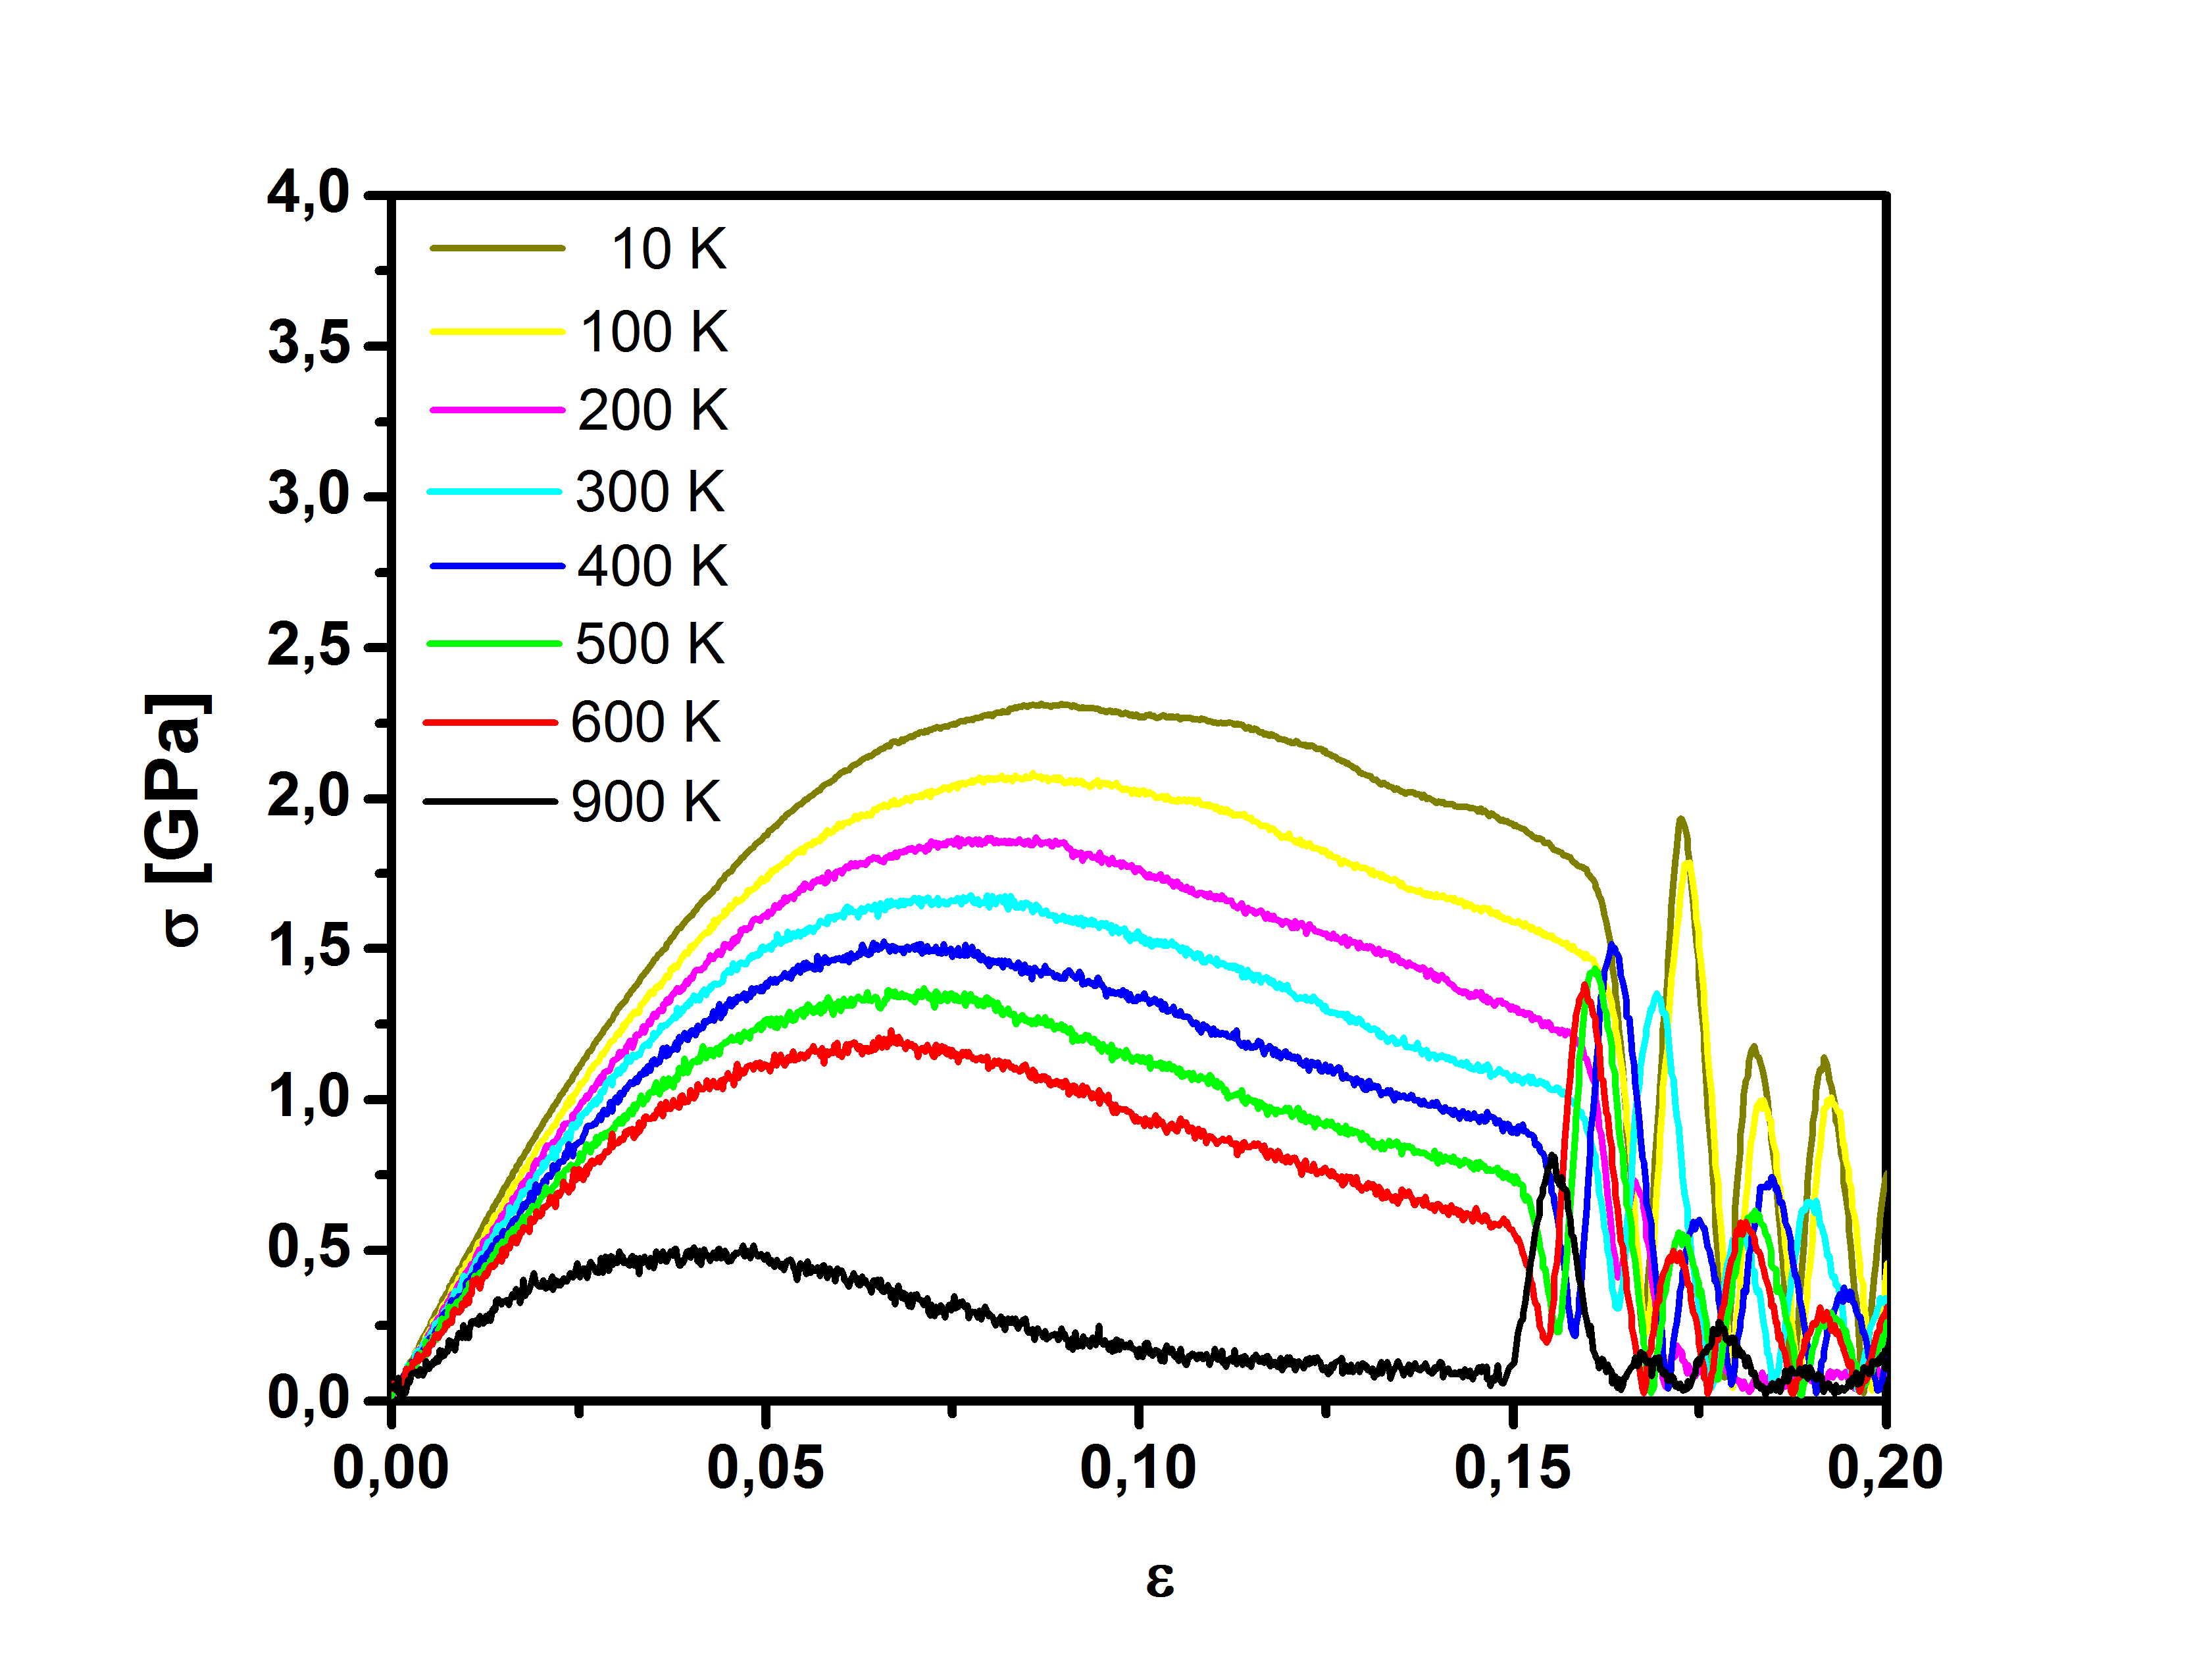
\includegraphics[width=10cm]{Cap_3/stress_strain_TEN.png}
	\label{C3:fg:sStrainTen}}
\\
\subfloat[Compression]{
	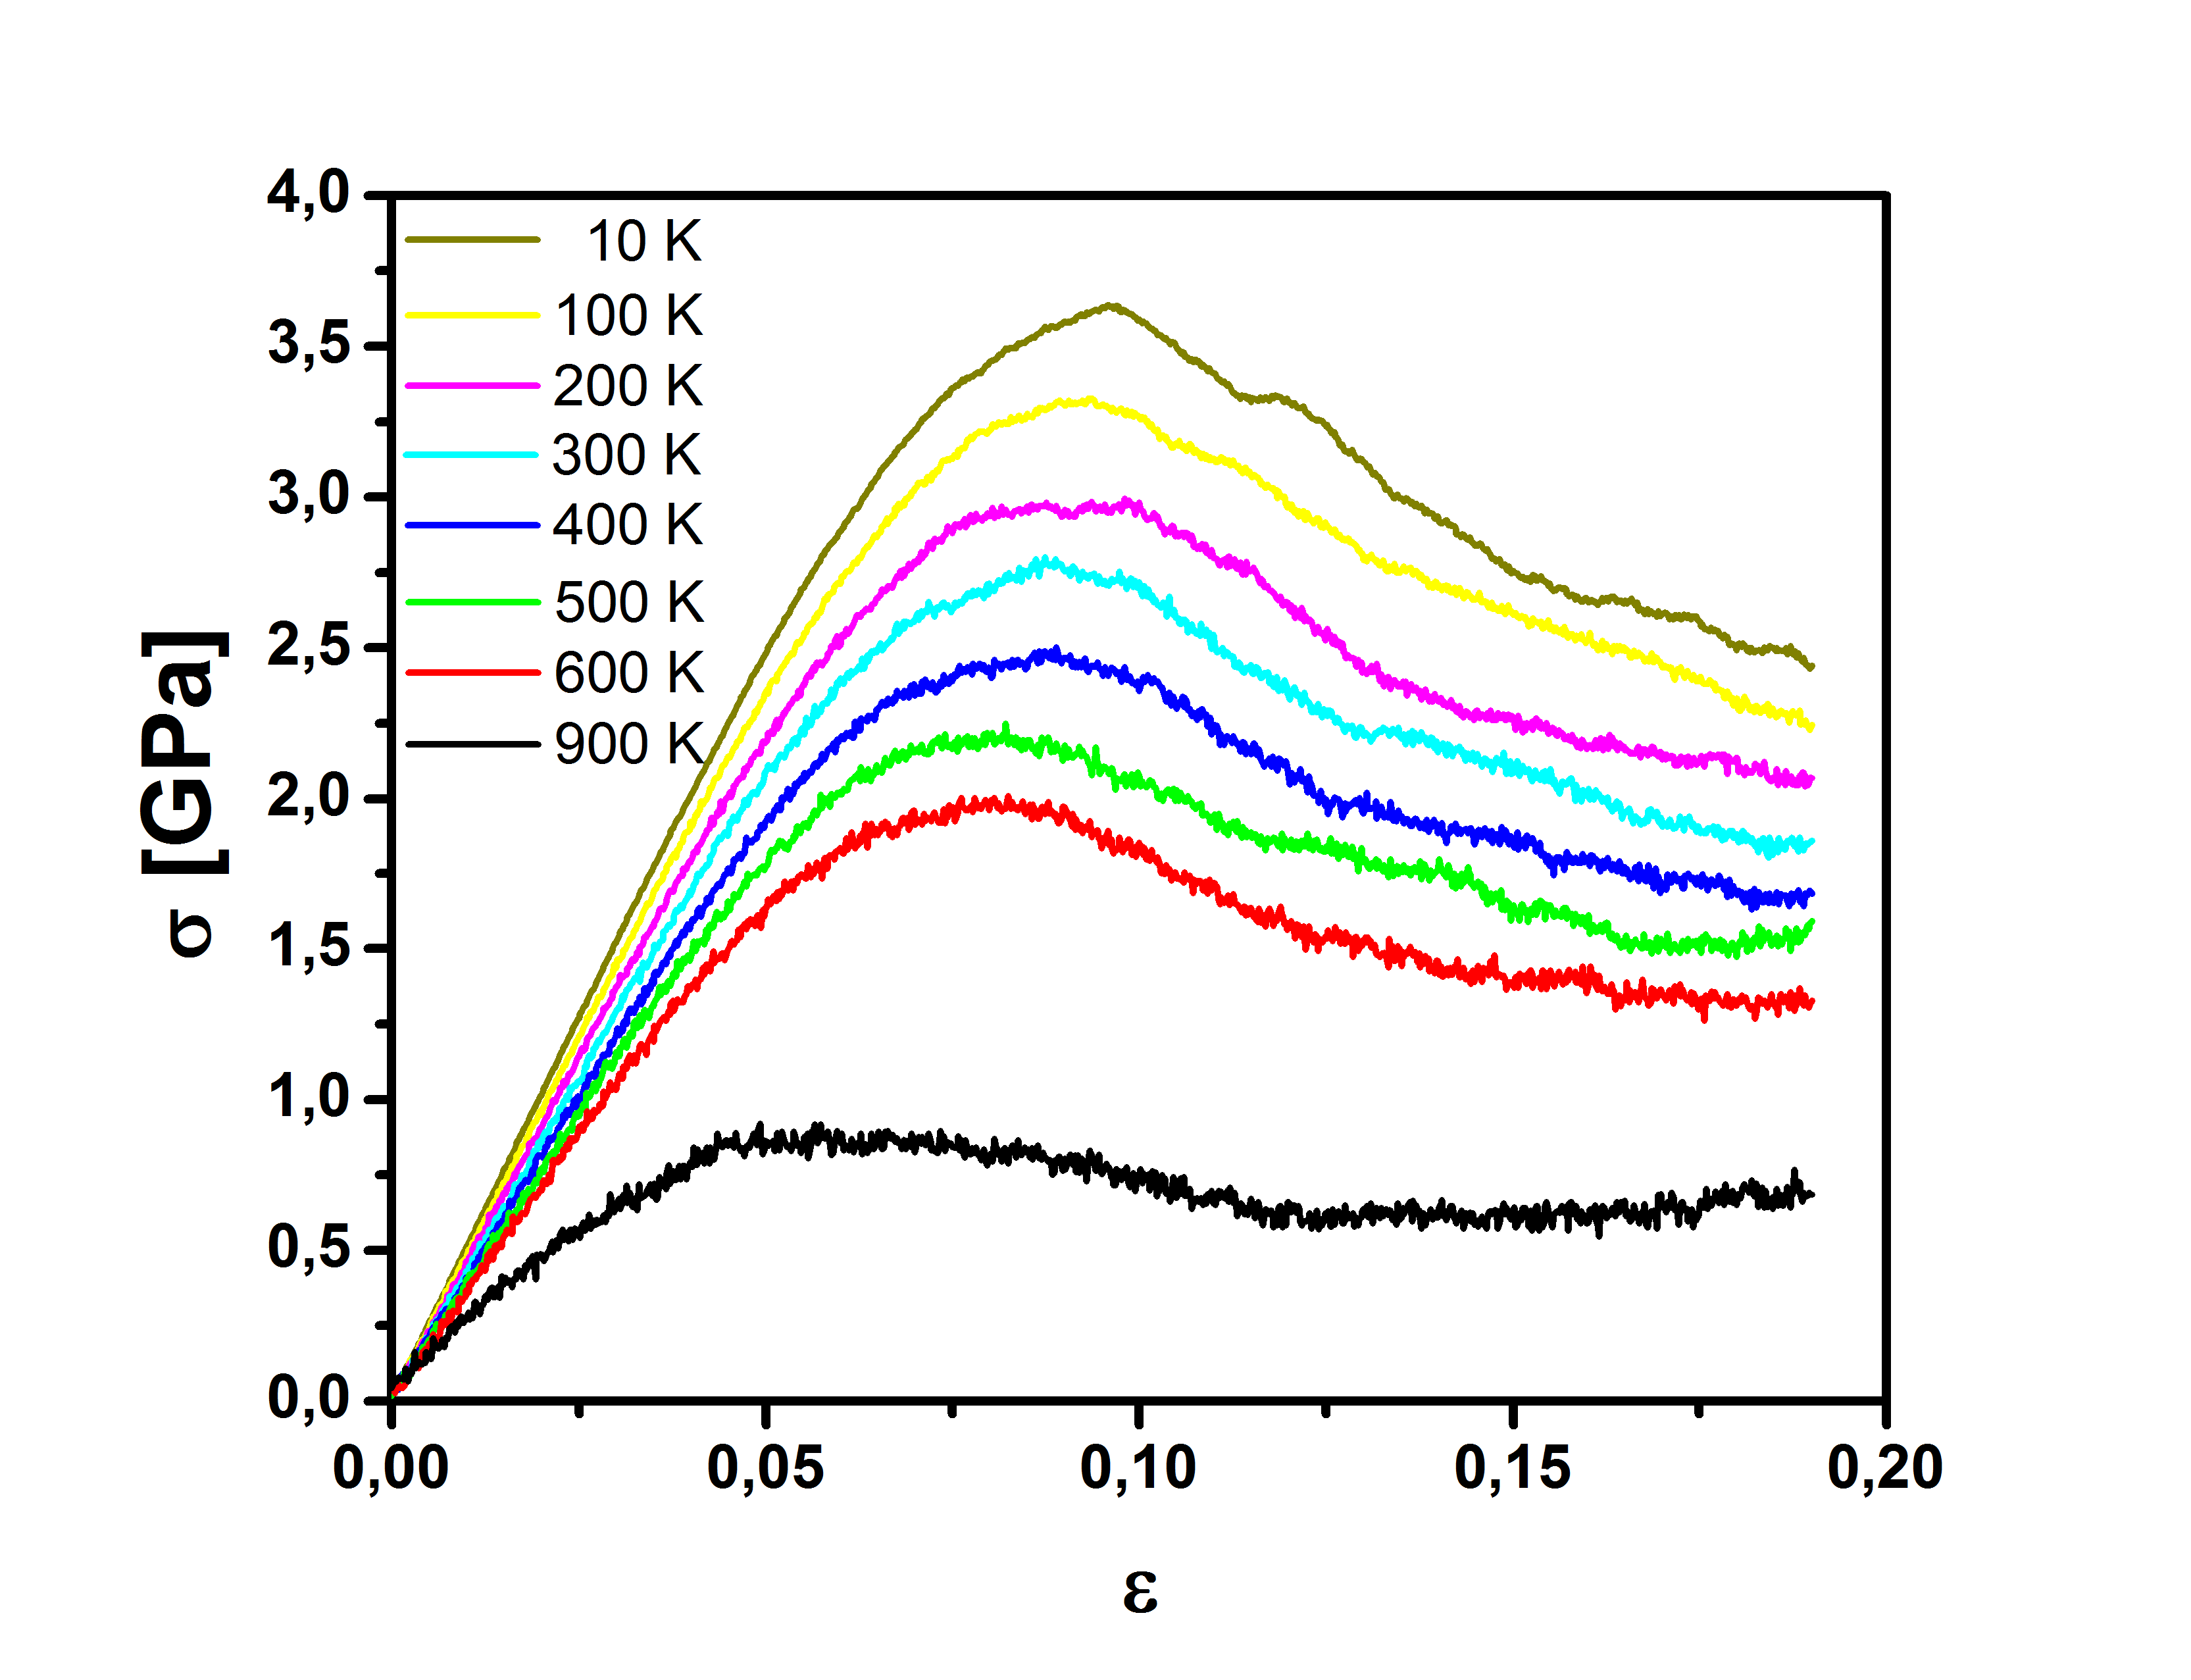
\includegraphics[width=10cm]{Cap_3/stress_strain_COMP.png}
	\label{C3:fg:sStrainComp}}
\caption{Stress-strain curves at different temperatures. (a) Tension (b) Compression. In tension, there are huge stress fluctuations starting with void nucleation near 15\% strain.}
\label{figure:msd_Cu}
\end{figure}

\begin{figure}[htp]
\centering
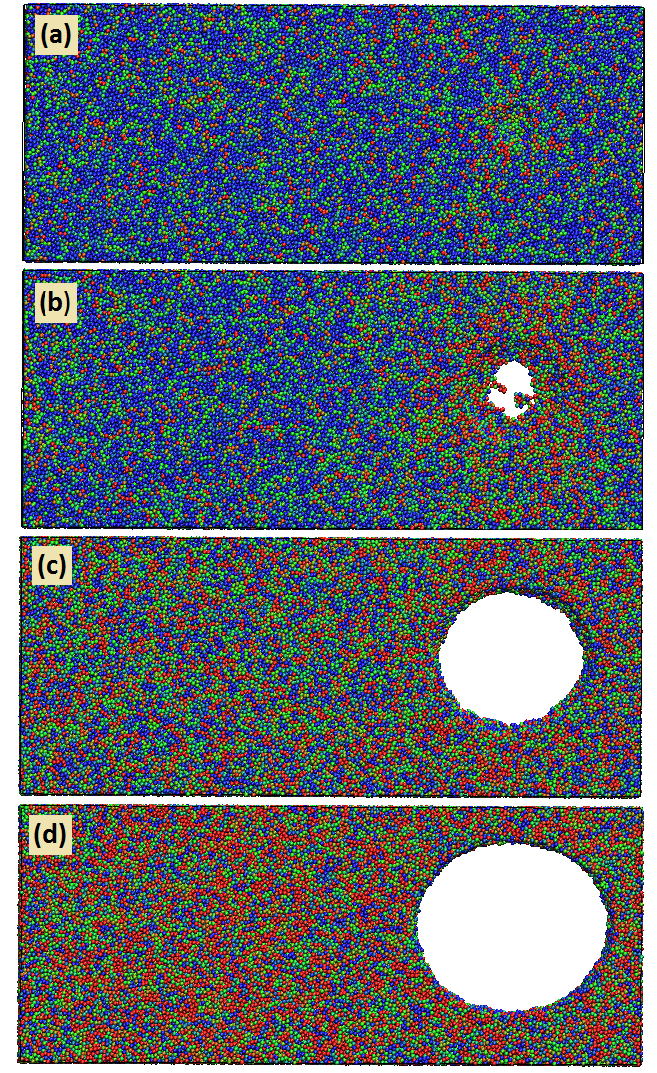
\includegraphics[width=10cm]{Cap_3/void_sequence.png}
\caption{Void nucleation in tension at temperature of 900 K. (a) $\epsilon$ = 0.137 (b) $\epsilon$ = 0.141 (c) $\epsilon$ = 0.145 (d) $\epsilon$ =0.149. Colors represent von Mises stress, red being high and blue low stress. Similar void nucleation is observed at lower temperatures.}
\label{C3:fg:voidSeq}
\end{figure}

We calculate mechanical properties, and propose the following simple functional form as an approximation for the thermal behavior:

\begin{eqnarray}
y = A_{1}\cdot \mathrm{e}^{\frac{-T}{T_{0}}}
\label{C3:eq:thermalFit}
\end{eqnarray}
	
where $A_{1}$ and $T_{0}$ are parameters. This functional form is often used for thermally activated phenomena. In Tables 2-3 we present the values for the coefficients of equation (1) obtained from the curves shown in Figures 3-6. It can be seen that the fits are reasonable. The correlation coefficient (R2) is greater than 0.9 in all cases, thus making our simple functional fit reasonable. Of course, further studies including many more temperature values are needed to truly test the fits. 

\begin{table}[htp]
\caption{Fit coefficients for tension.}
\begin{center}
\begin{tabular}{*{4}{c}}
Tracción & Parámetros & Valor & $R^{2}$ \\
Peak von Mises stress & A$_{1}$ & 2.312 $\pm$ 0.055 & 0.989 \\
 & T$_{0}$ & 1059.6 $\pm$ 68.8 & \\
von Mises stress ($\epsilon$=0.12) & A$_{1}$ & 2.23 $\pm$ 0.22 & 0.935 \\
 & T$_{0}$ & 509.4 $\pm$ 101.7 & \\
Young Modulus & A$_{1}$ & 51.3 $\pm$ 2.6 & 0.928 \\
 & T$_{0}$ & 1419.5 $\pm$ 239.0 & \\
Yield Stress & A & 0.0604 $\pm$ 0.004 & 0.952 \\
 & B & -0.041 $\pm$ 0.005 & 
\end{tabular}
\end{center}
\label{C3:tb:initPropsTen}
\end{table}

\begin{table}[htp]
\caption{Fit coefficients for compression.}
\begin{center}
\begin{tabular}{*{4}{c}}
Compresión & Parámetros & Valor & $R^{2}$ \\
Peak von Mises stress & A$_{1}$ & 3.77 $\pm$ 0.23 & 0.931 \\
 & T$_{0}$ & 804.3 $\pm$ 144.2 & \\
von Mises stress ($\epsilon$=0.18) & A$_{1}$ & 2.58 $\pm$ 0.22 & 0.915 \\
 & T$_{0}$ & 863.6 $\pm$ 166.6 & \\
Young Modulus & A$_{1}$ & 52.14 $\pm$ 1.61 & 0.972 \\
 & T$_{0}$ & 1437.7 $\pm$ 146.8 & \\
Yield Stress & A & 0.123 $\pm$ 0.01 & 0.930 \\
 & B & -0.081 $\pm$ 0.013 & 
\end{tabular}
\end{center}
\label{C3:tb:initPropsComp}
\end{table}

As expected, the elastic modulus, peak von Mises stress and yield stress, all decrease with increasing temperature. We obtained a smooth behavior even when T is above Tg, as seen in Figures 3-6.

\begin{figure}[htp]
\centering
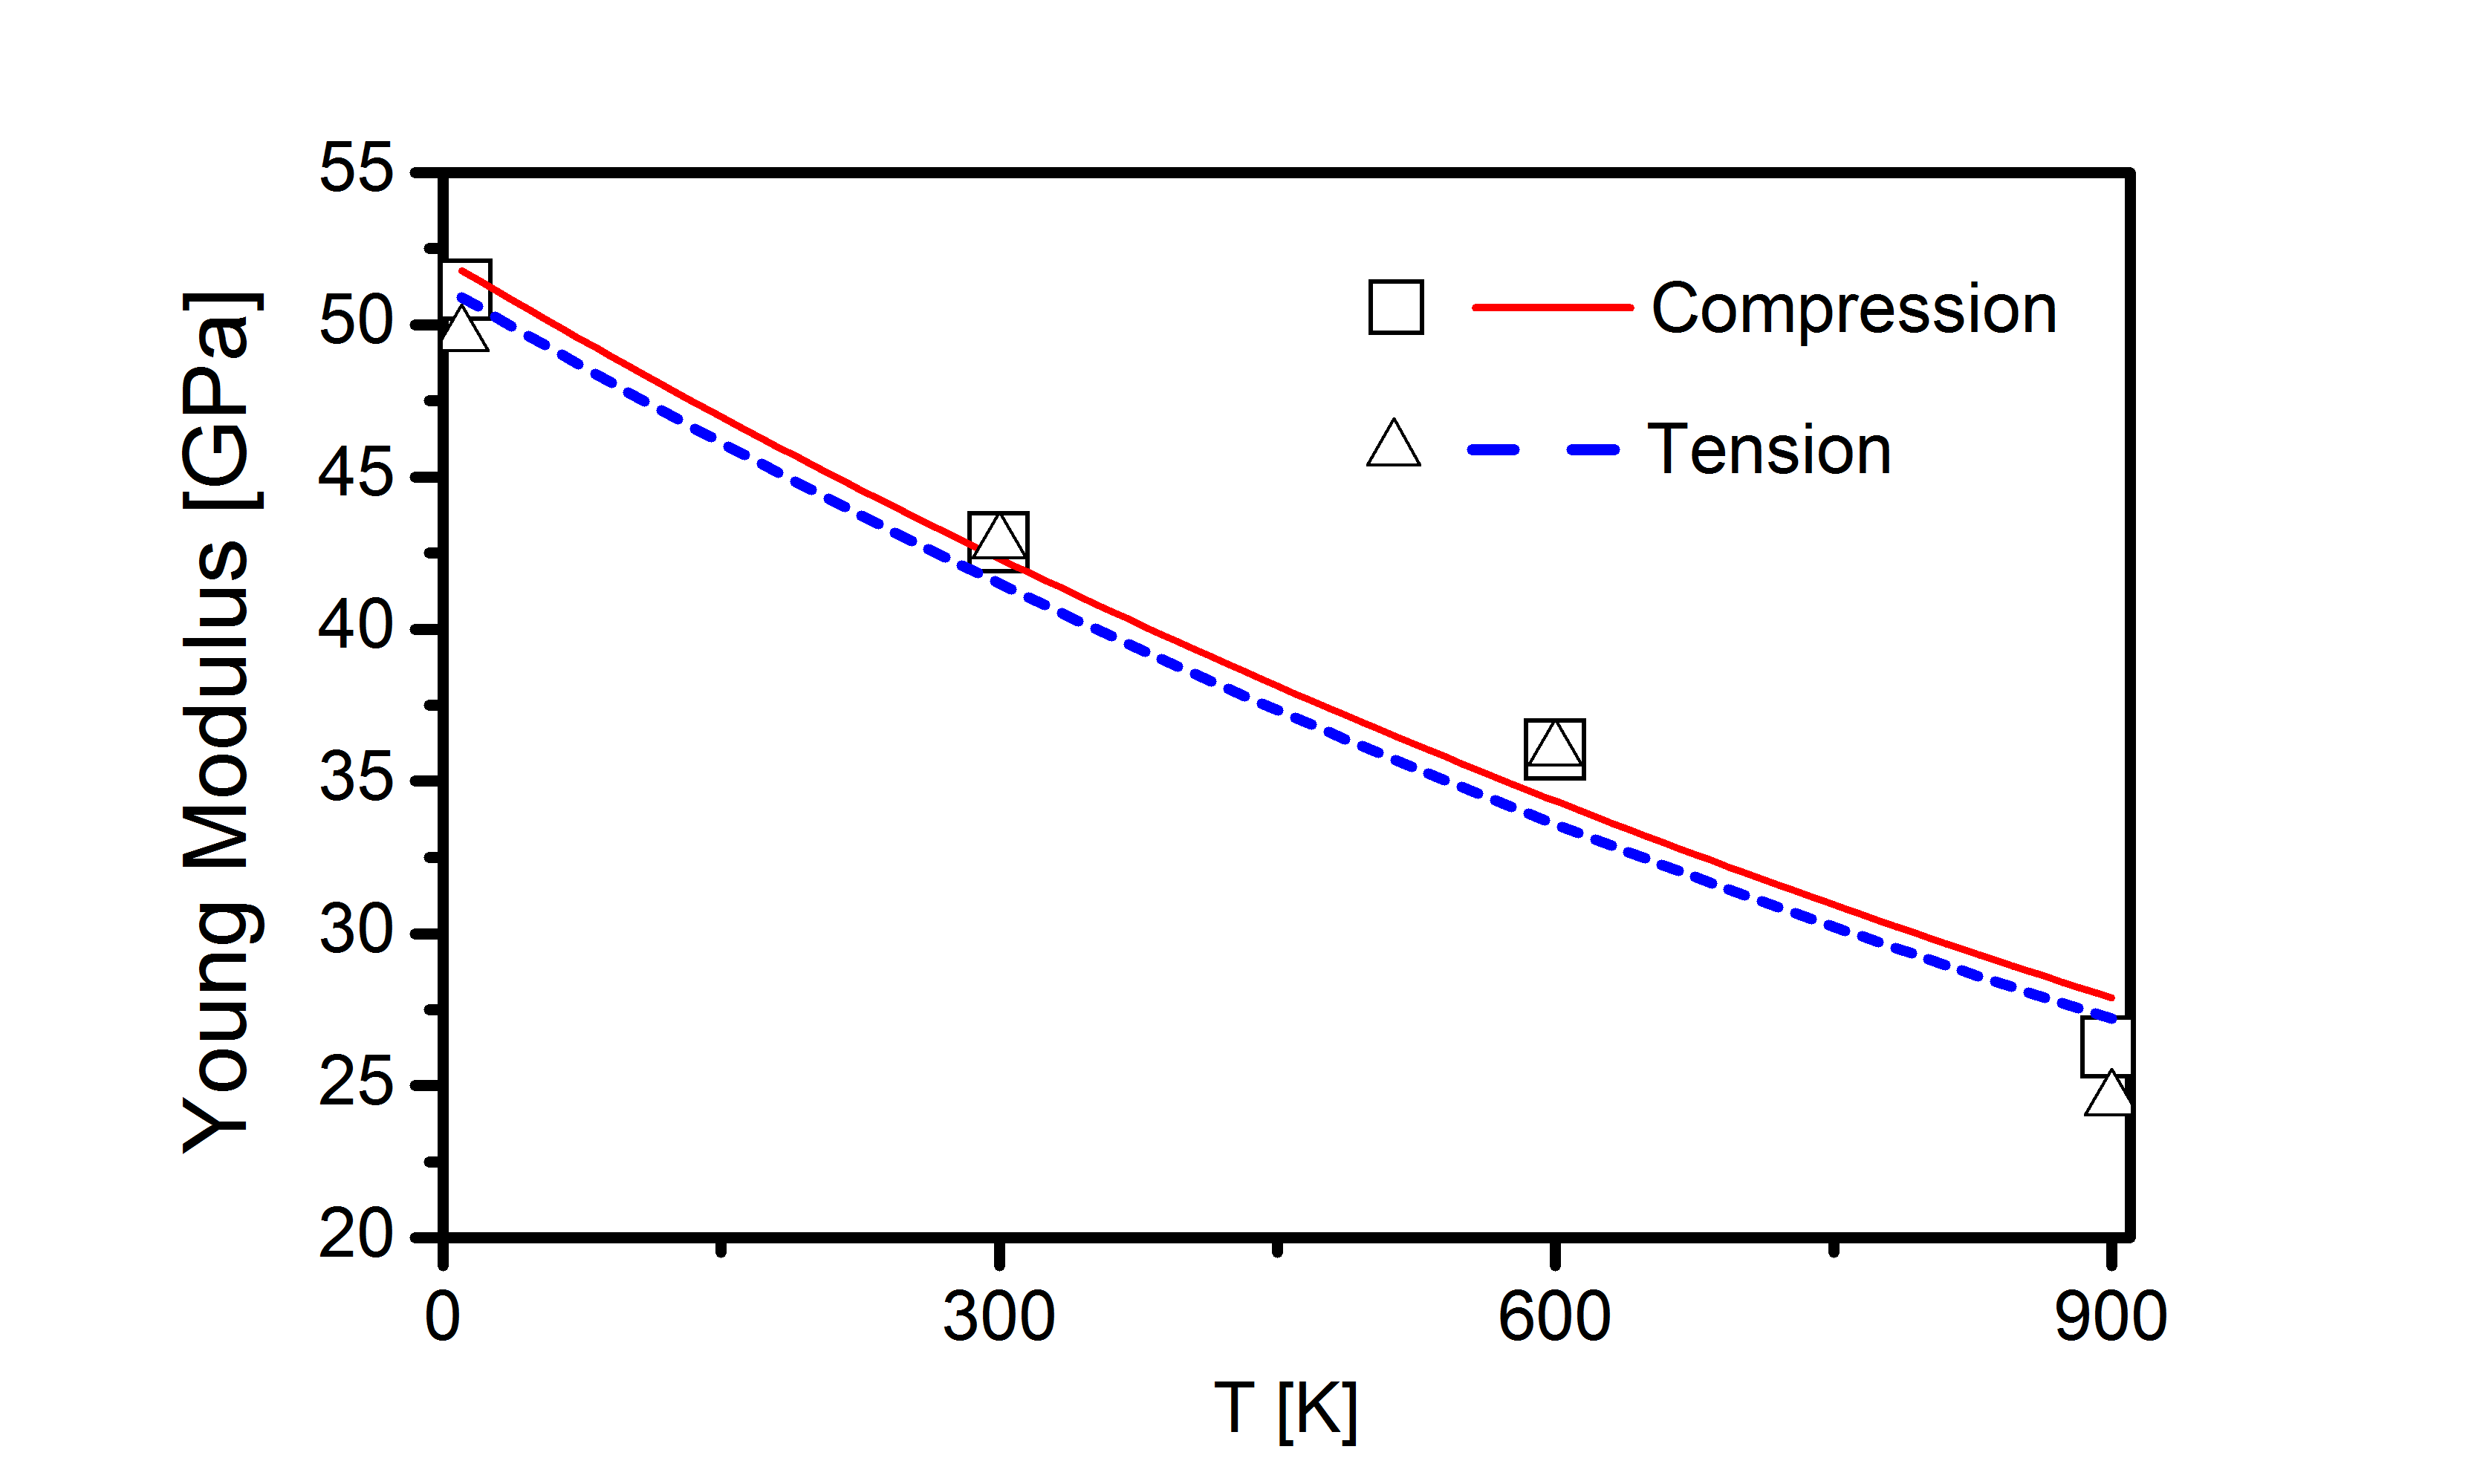
\includegraphics[width=10cm]{Cap_3/FitYoungBoth.png}
\caption{Young modulus variation with temperature.}
\label{C3:fg:youngVsT}
\end{figure}

\begin{figure}[htp]
\centering
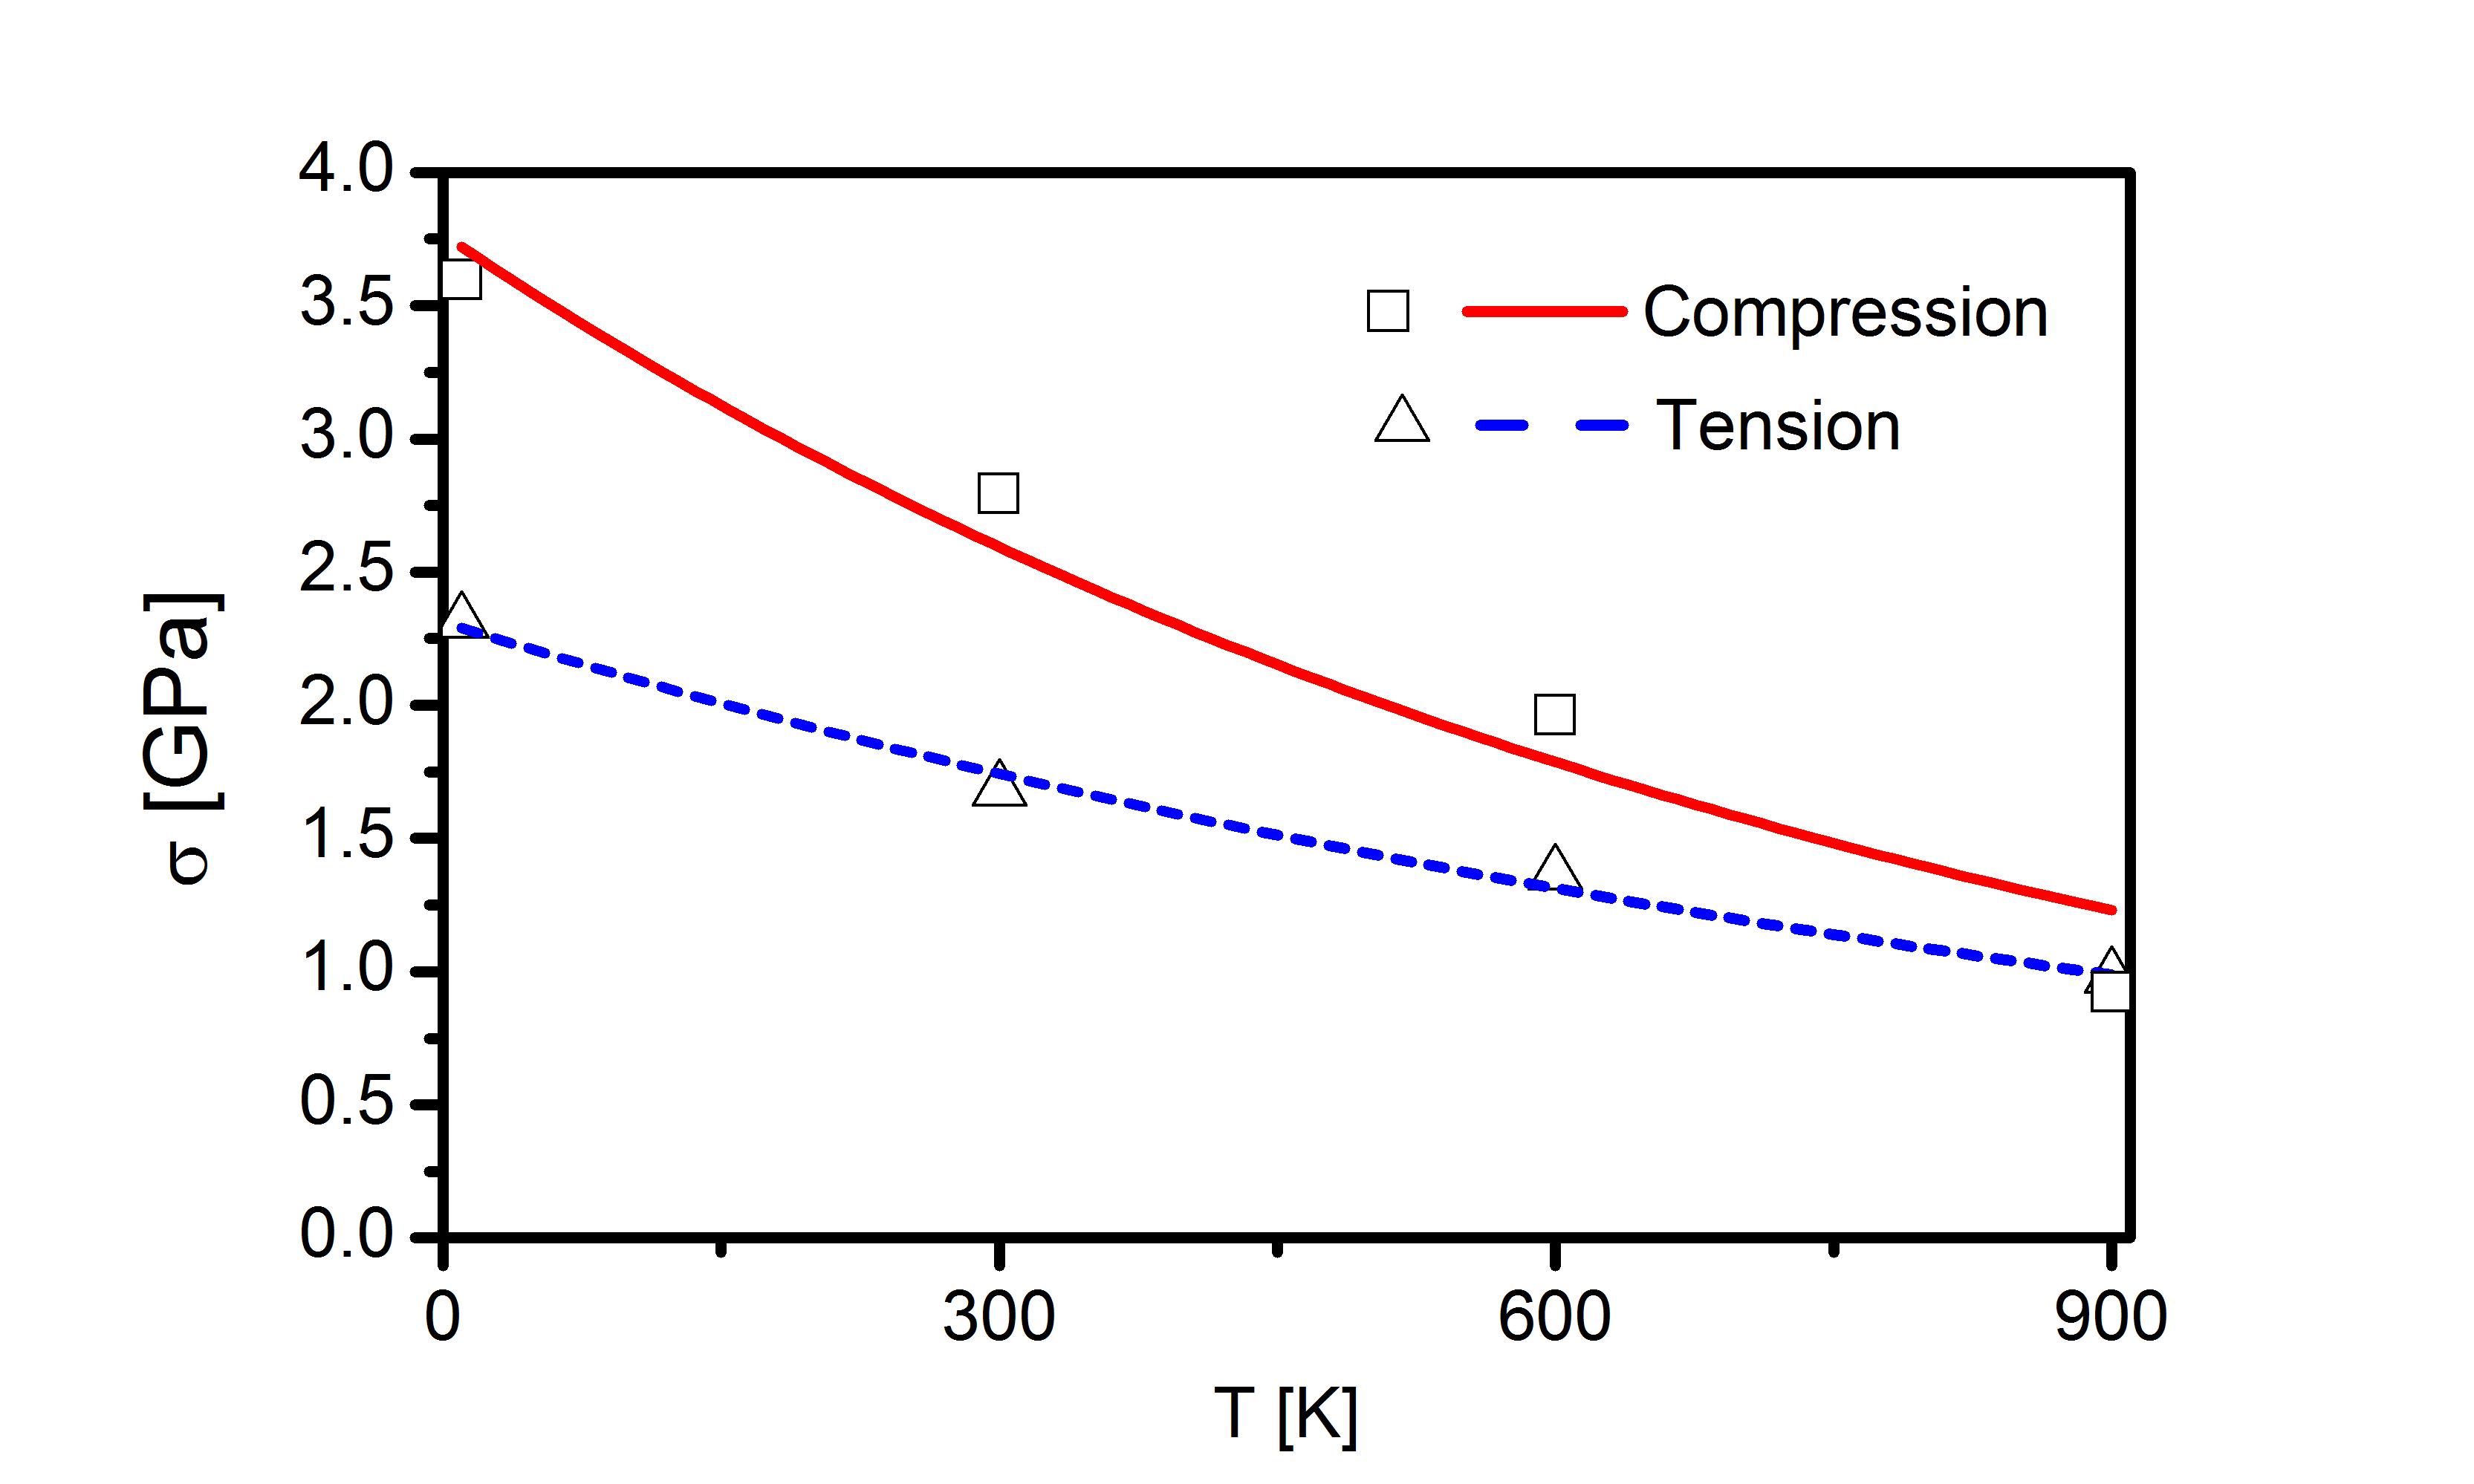
\includegraphics[width=10cm]{Cap_3/FitPeakBoth.png}
\caption{Peak von Mises stress variation with temperature.}
\label{C3:fg:peakVMisesVsT}
\end{figure}

\begin{figure}[htp]
\centering
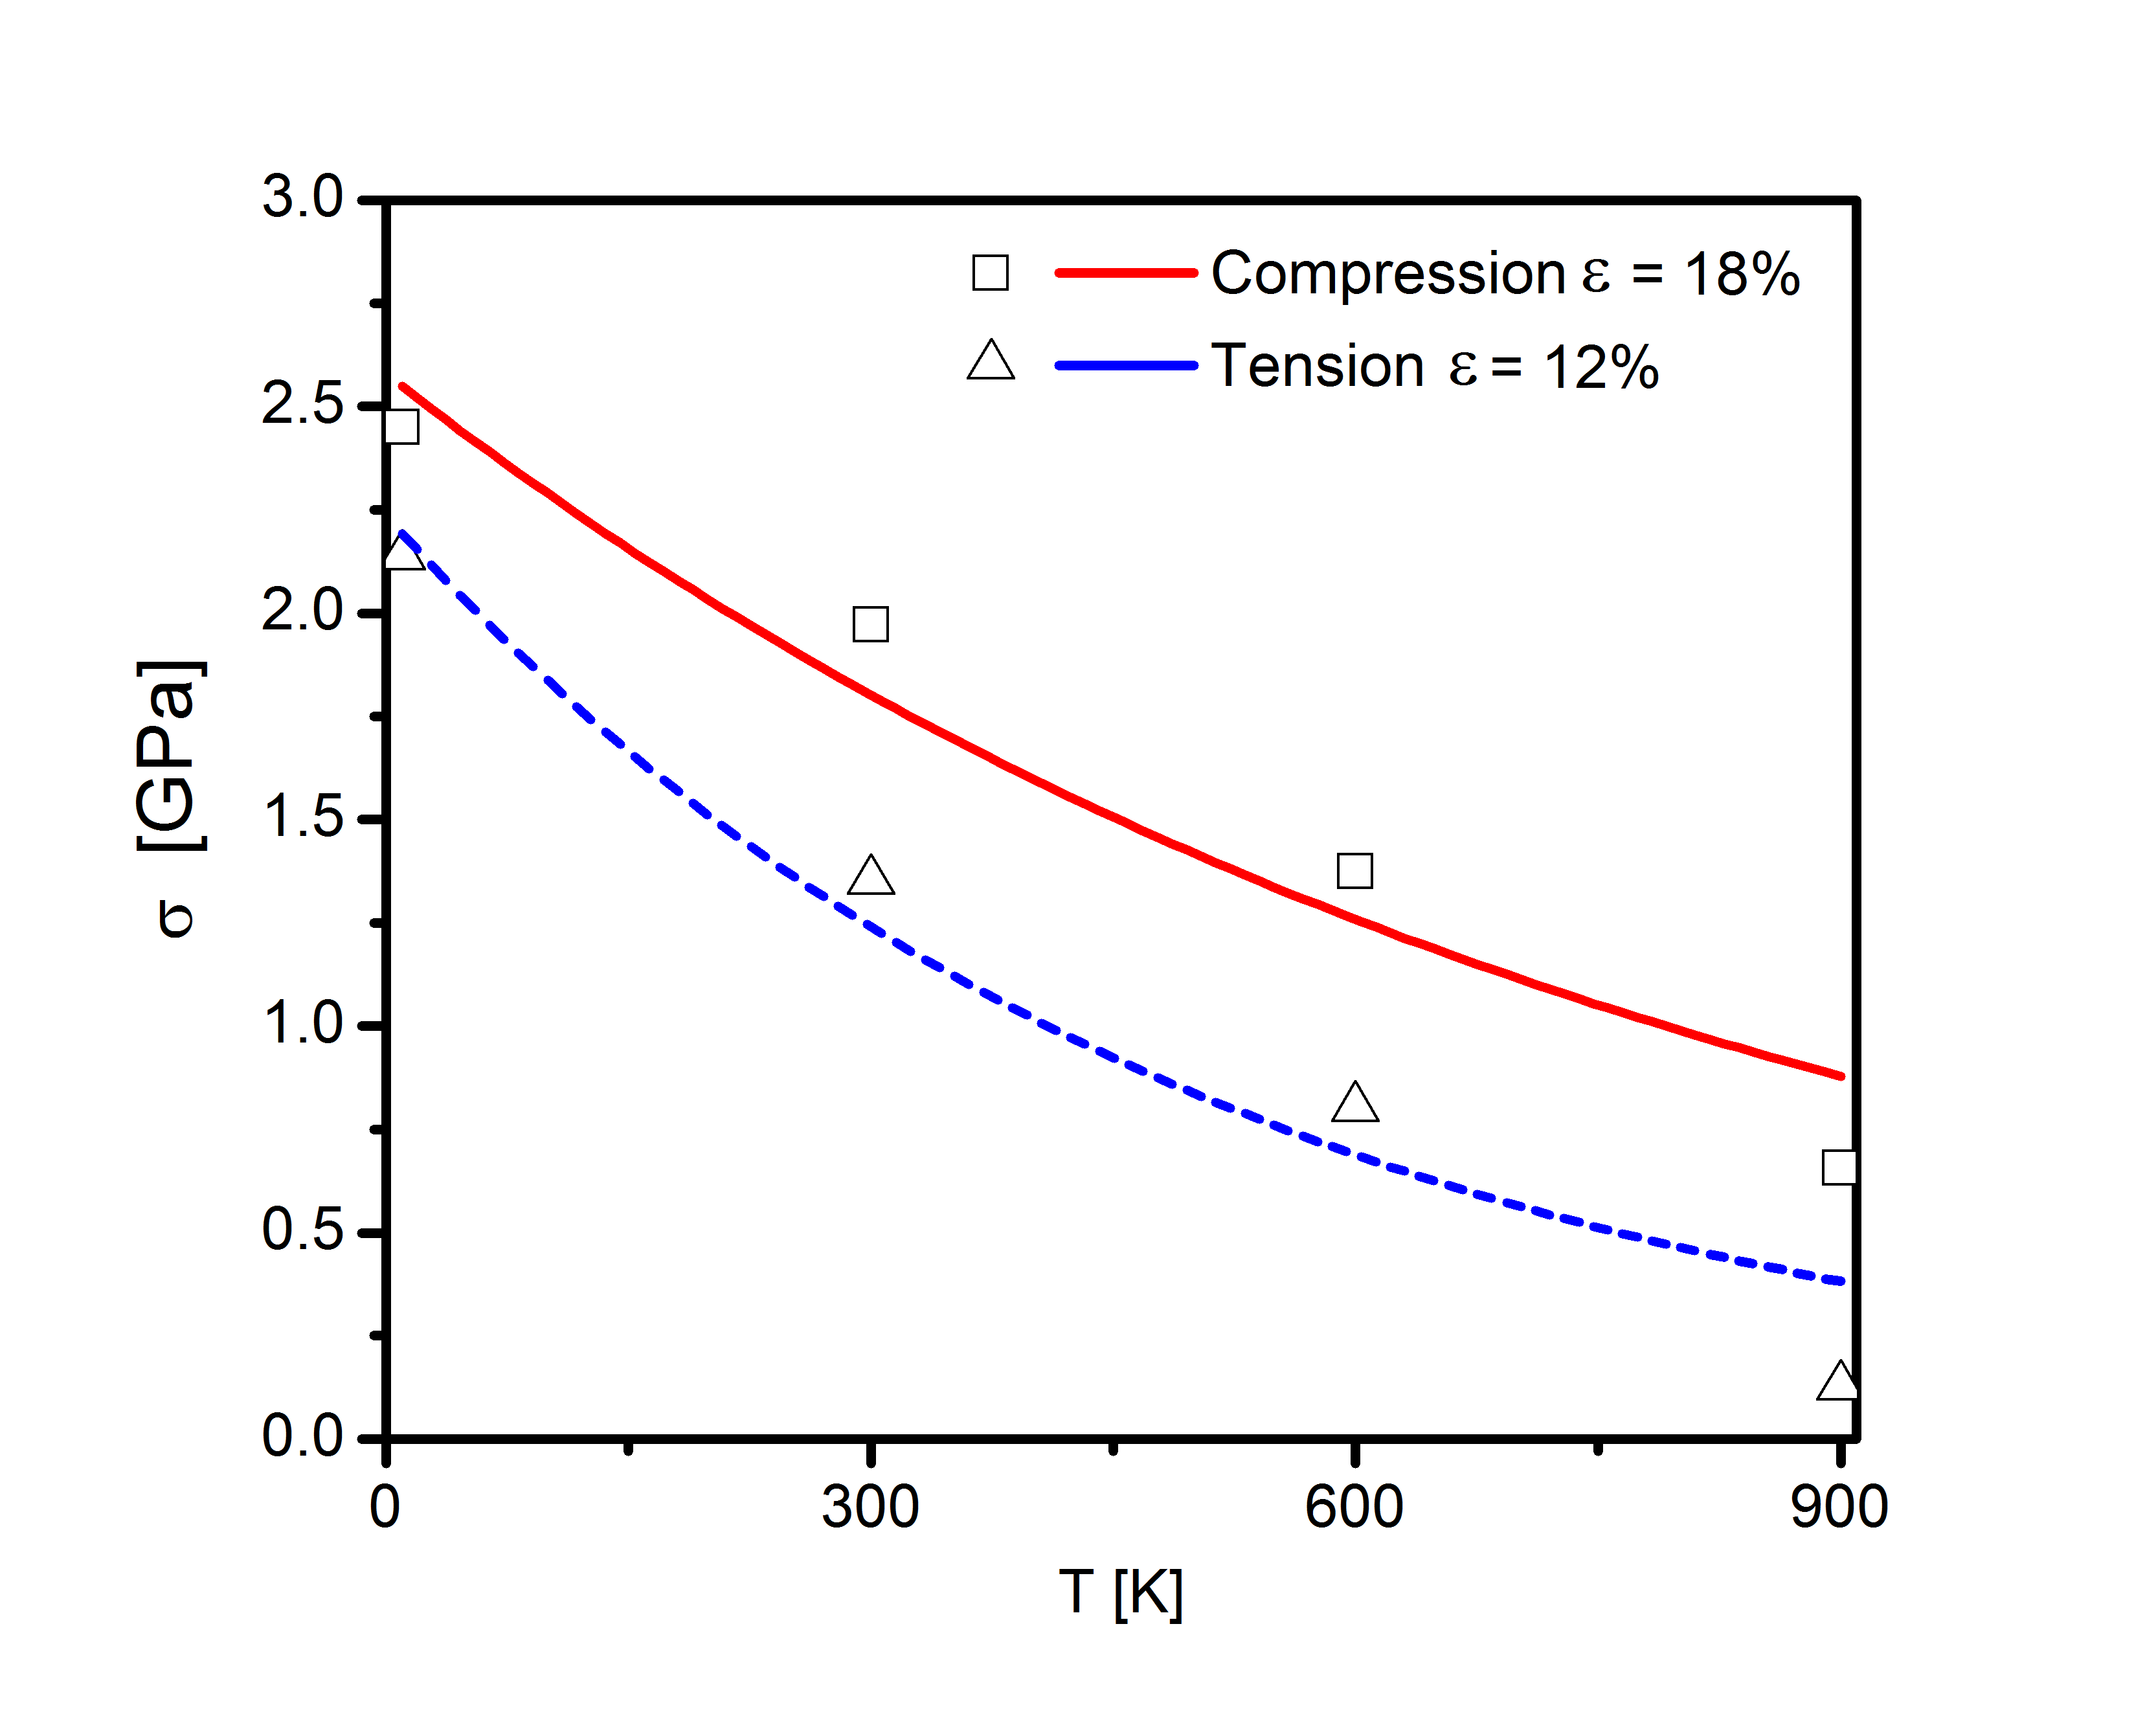
\includegraphics[width=10cm]{Cap_3/Fit1218.png}
\caption{von Mises stress variation with temperature. The lower strain used in tension is to avoid stress fluctuations due to void nucleation.}
\label{C3:fg:peakVMises1218VsT}
\end{figure} 

Cheng et al. (2011) attempted to describe the behavior of the onset of plasticity under pure shear, as a function of several variables, including temperature, based on a CSM (cooperative shear model). The resulting temperature dependence was (T/Tg)2/3, and we try to apply this behavior to our results. Simplifying the expression in Cheng et al. (2011), we obtain the following expression:

\begin{eqnarray}
\frac{\sigma{}_{y}}{G} = A+B(\frac{T}{Tg})^{2/3}
\label{C3:eq:onsetPlast}
\end{eqnarray}

where $\sigma{}_{y}$ is the yielding stress, while A and B are parameters of the fit. To obtain the yield stress in our simulations we assume that plasticity starts when the stress-strain curve departs 20\% from the linear elastic behavior extrapolated from very low strains (below $\epsilon$=1\%). In Tables 2-3 we present the values for the coefficients of equation (2) obtained for the curves shown in Figure 6. In this figure we compare the fittings for tension and compression with the result from Johnson and Samwer (2005), who obtained, for experiments under pure shear deformation the following expression:

\begin{eqnarray}
\frac{\tau _{y}}{G} = 0.036-0.016(\frac{T}{Tg})^{0.62}
\label{C3:eq:johnsonSamwer}
\end{eqnarray}
	
where $\tau _{y}$ is the shear yield strength .We observe that equation (2) fits both uniaxial tension and compression quite well. There are discrepancies with the experimental fit from equation (3), but we note that the coefficients in that fit had large error bars, and data showed large dispersion. For instance, the exponent was 0.62 $\pm$ 0.2.

\begin{figure}[htp]
\centering
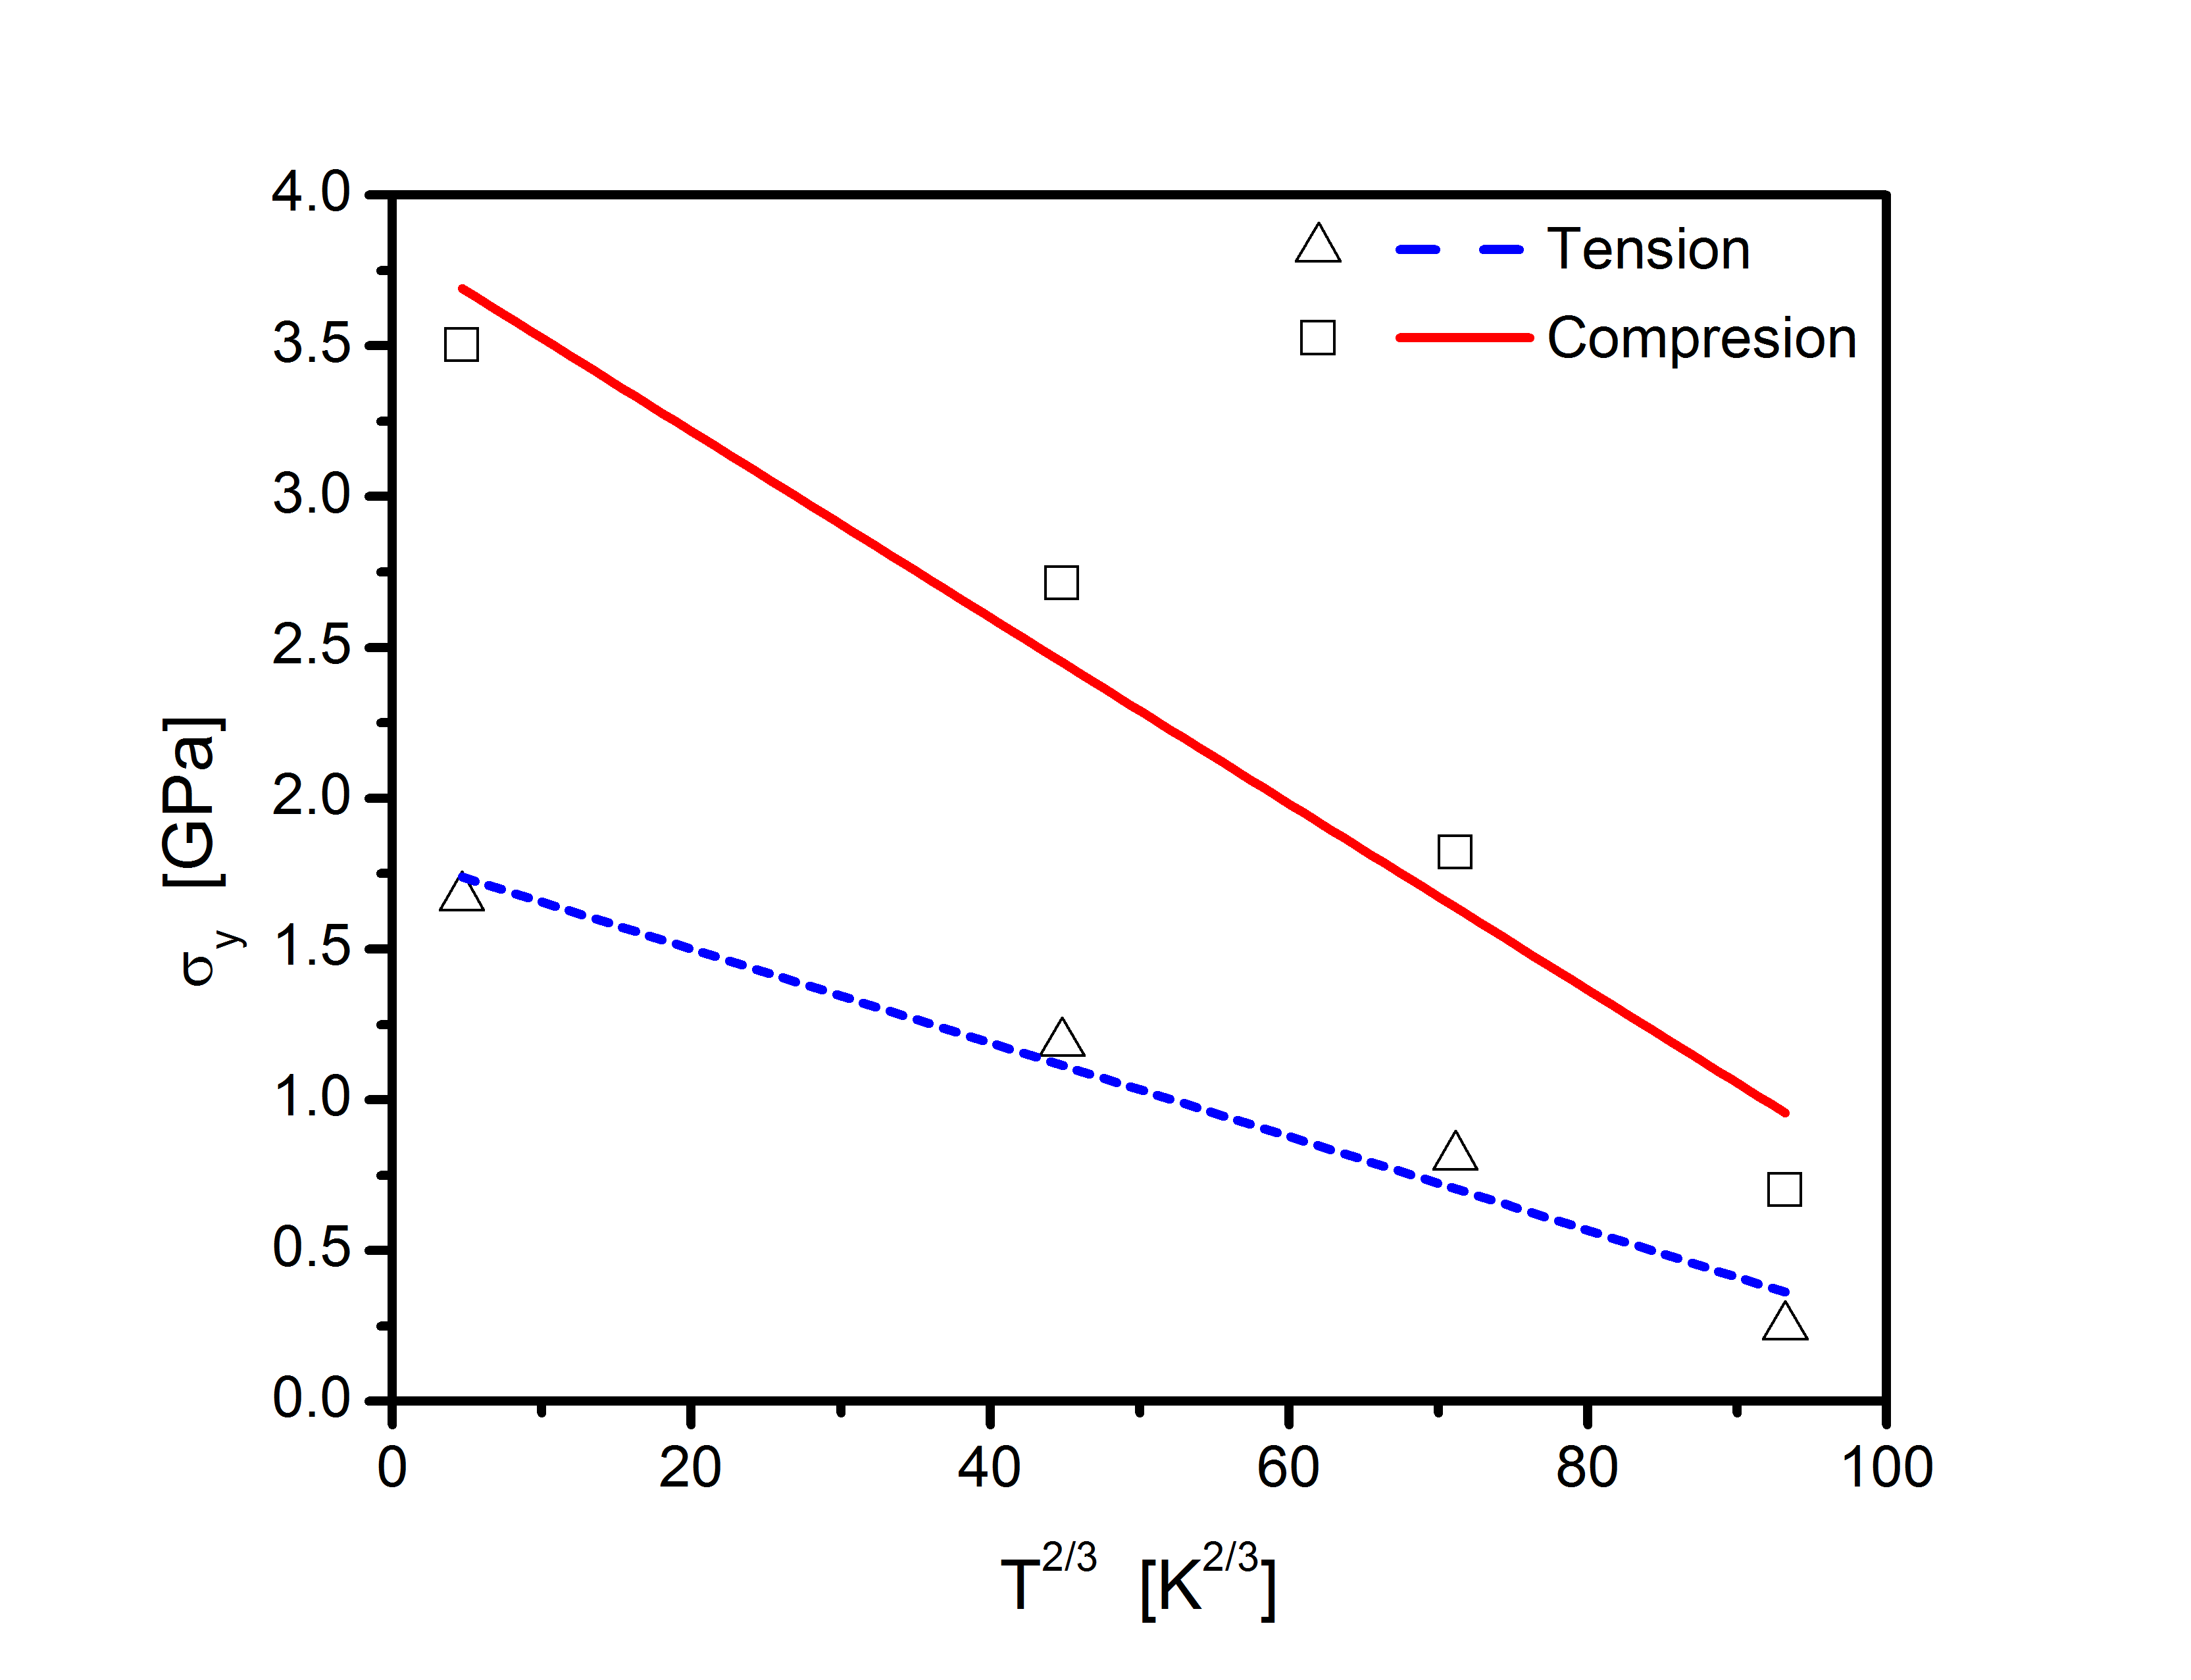
\includegraphics[width=10cm]{Cap_3/Fitdostercios.png}
\caption{Yield Stress variation with temperature. We use the experimental values of Tg and G from experiments (Johnson and Samwer, 2005) to normalize our results.}
\label{C3:fg:fitDosTercios}
\end{figure}

Figure 7 shows atomic von Mises stress for the complete sample in the case of tension at T=300K. Despite the evidence of plastic behavior in stress-strain curves, we do not observe evidence of shear bands.

According to a recent study in metallic glass nanowires (Xiao et al., 2012), the presence of shear bands strongly depends on the quenching rate of the glass. In this case, for the quenching rates used in the creation of our sample, shear bands should not be observed, as shown in Figure 7.

\begin{figure}[htp]
\centering
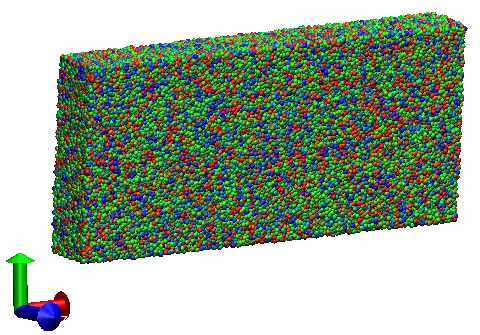
\includegraphics[width=10cm]{Cap_3/All_300K_6pstrain_sacale100-280_Trac.png}
\caption{View of our  sample, at $\epsilon$=6\%, under uniaxial tension, at T=300 K. Colors represent von Mises stress, red being high and blue low stress. The stress scale ranges from 100 GPa to 280 GPa. No shear bands are observed. Visualization made with VMD (Humphrey et al., 1996). Similar results are found at the other simulated temperatures.}
\label{C3:fg:sampleTen}
\end{figure}

When the metallic glass deforms under uniaxial compression we can observe a similar behavior in the stress-strain curves shown in Figure 1 (b) to the curves corresponding to tension in Figure 1 (a), for strains below 15\%. However, since there is no void nucleation above 15\%, the behavior of the curves is smooth even at very high strains.

Figures 3-6 show the same type of fit that the one used for tension, and there is also a reasonable adjustment, even with the simple functional form shown in equation (1).

Figure 8 shows that, similarly to the sample under tension, no shear bands are observed, as expected given the high quenching rate of the glass used here.

\begin{figure}[htp]
\centering
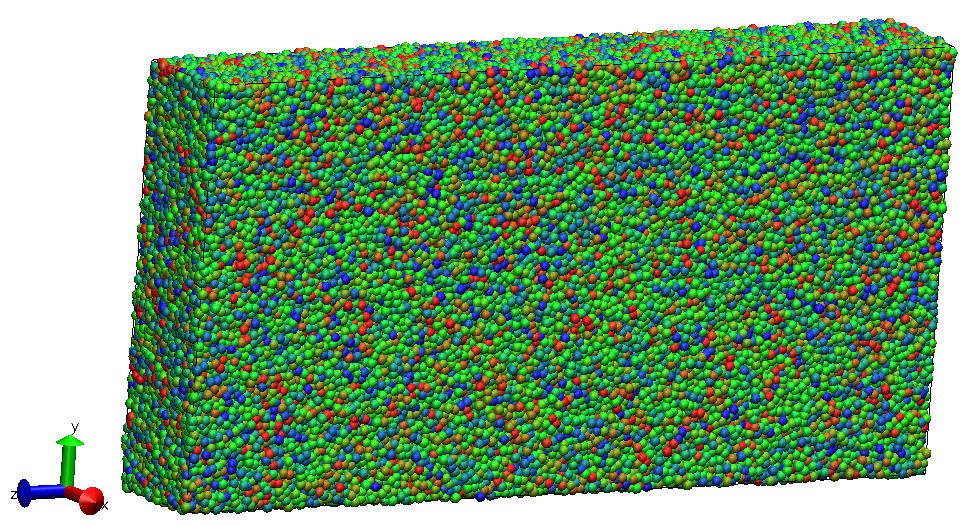
\includegraphics[width=10cm]{Cap_3/All_300K_6pstrain_sacale100-400_Comp.png}
\caption{View of our sample, at $\epsilon$=6\%, under uniaxial compression, at T=300 K. Colors represent von Mises stress, red being high and blue low stress. The stress scale ranges from 100 GPa to 400 GPa. No shear bands observed. Visualization made with VMD (Humphrey et al., 1996). Similar results are found at the other simulated temperatures.}
\label{C3:fg:sampleComp}
\end{figure}

\subsection{Tension-compression asymmetry}

To highlight the differences between tension and compression, Figure 9 shows that elastic modulus are almost equivalent under tension or compression, but that the maximum values of the von Mises stress have great differences, except at very high temperature (above Tg). Tension-compression asymmetries are expected in amorphous materials, which have a yield surface that follow a Mohr-Coulomb law (Schu et. al, 2003).

\begin{figure}[htp]
\centering
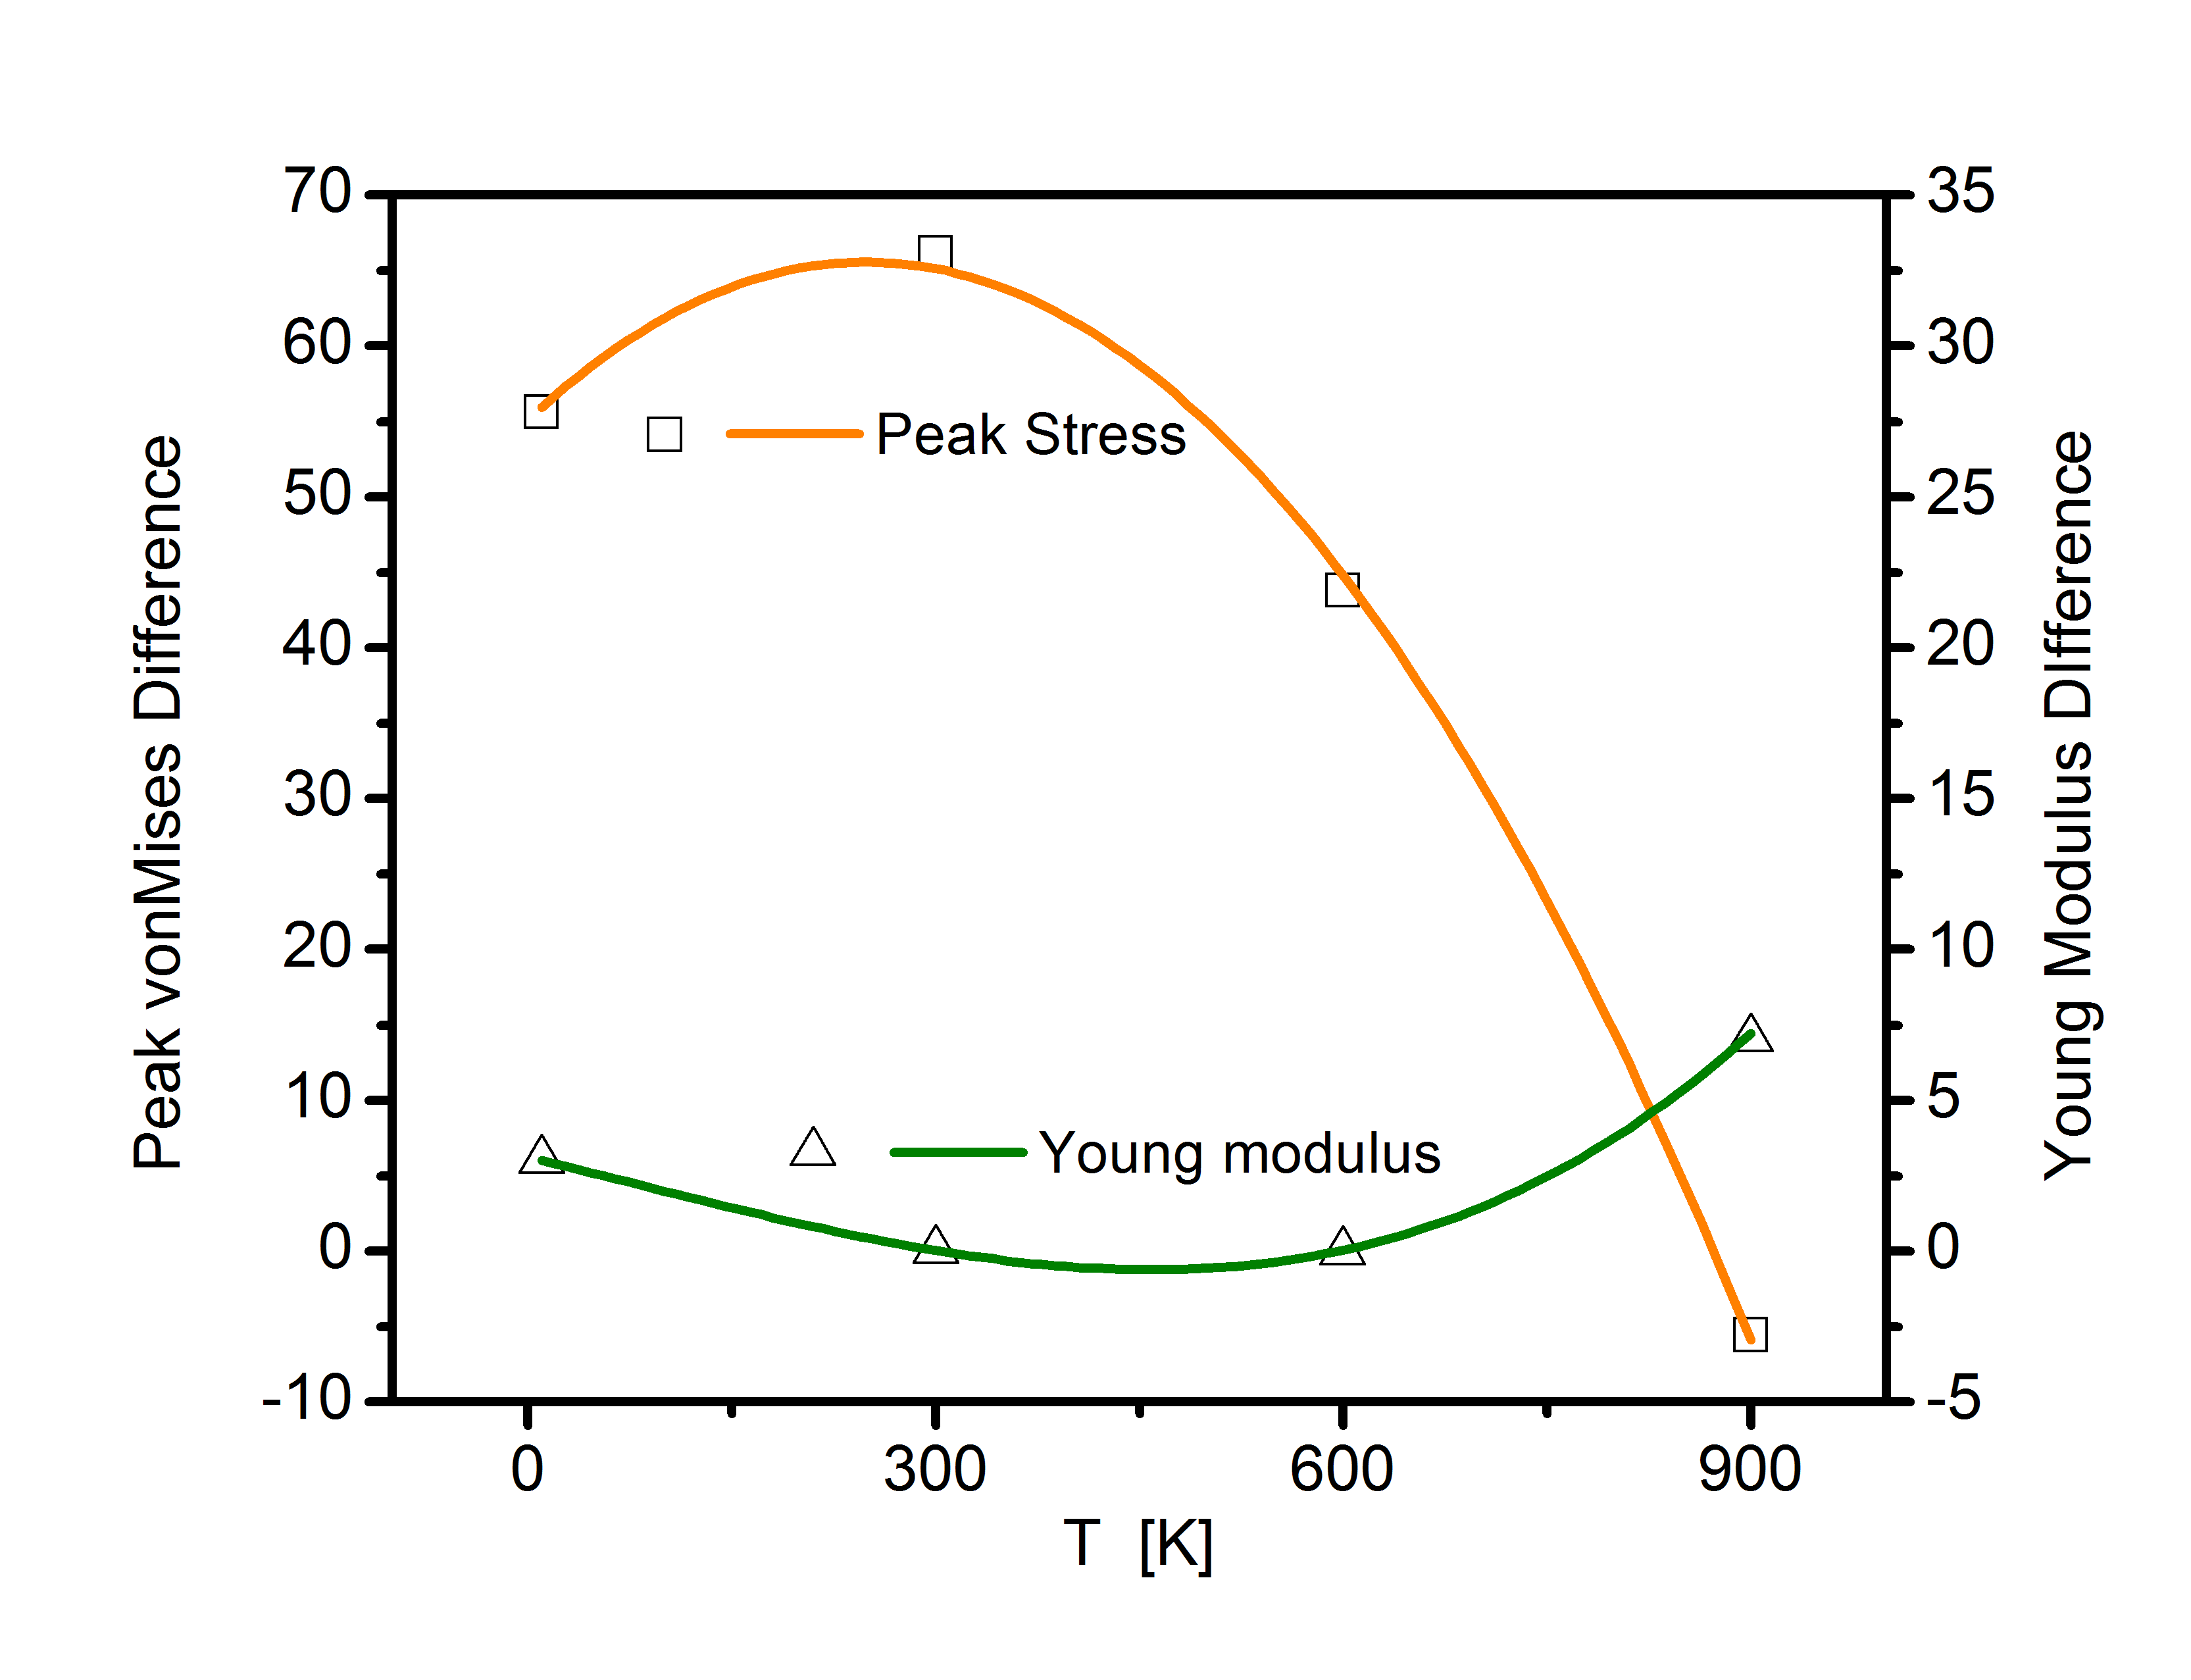
\includegraphics[width=10cm]{Cap_3/Peak_YoungDif.png}
\caption{Percentage difference (between compression and tension values, assuming tension values as basis) of Young modulus and peak von Mises stress. Lines are just for visualization.}
\label{C3:fg:peakYoungDif}
\end{figure}

\subsection{Simulation of the sample with free boundary conditions}

To verify that the absence of shear bands is not due to periodic conditions during deformation, simulations were carried out with free lateral boundary conditions, as shown in Figure 10. Under tension there is a slight decrease in the cross section of the sample, as expected. This is shown in Figure 11. We can also observe that the shape of the cross section has changed from rectangular to elliptical, due to surface energy minimization.

These simulations are similar to those of metallic glass nanowires seen in Xiao et al.(2012). Under compression, buckling is observed. In both cases there is a lack of shear bands, as expected with the cooling rates used in our samples.

\begin{figure}[htp]
\centering
\subfloat[Tension]{
	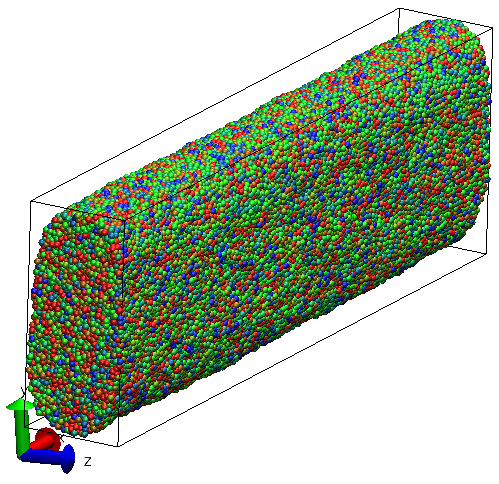
\includegraphics[width=10cm]{Cap_3/900libresTen.png}
	\label{C3:fg:libresTen}}
\\
\subfloat[Compression]{
	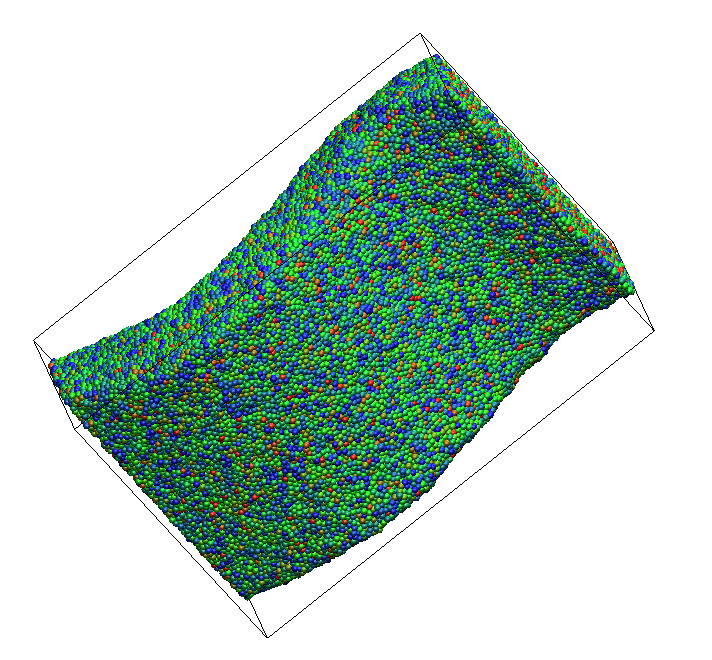
\includegraphics[width=10cm]{Cap_3/300libresComp.png}
	\label{C3:fg:libresComp}}
\caption{Tension and Compression simulations using free boundaries conditions. In both cases $\epsilon$=0.20 . In sample under uniaxial tension T=900K, and T=300K for the case of uniaxial compression. Necking is not observed, possibly because we are above Tg in this simulation.}
\label{C3:fg:libres}
\end{figure}

\begin{figure}[htp]
\centering
\subfloat[]{
	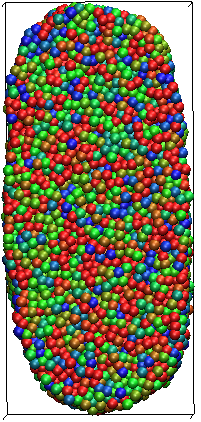
\includegraphics[width=10cm]{Cap_3/crossa.png}
	\label{C3:fg:crossExtreme}}
\\
\subfloat[]{
	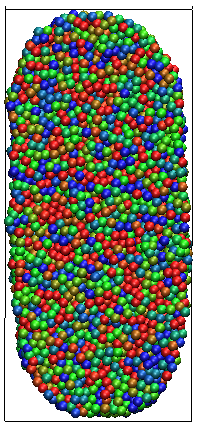
\includegraphics[width=10cm]{Cap_3/crossb.png}
	\label{C3:fg:crossMiddle}}
\caption{Cross section at different distances along the z axis, for the simulation showed in Figure 10. (a) Section close to the extreme. (b) Middle section. There is no appreciable necking of the sample, even at this large strain.}
\label{C3:fg:cross}
\end{figure}

\section{CONCLUSIONS}
Atomistic simulations of bulk metallic glasses (BMGs) mechanical behavior under tension and compression were performed using molecular dynamics (MD) simulations. The increase of sample temperature produces a considerable decrease of the samples elastic modulus. The same applies to maximum von Mises stress. It is observed that the elastic modules are practically the same under tension or compression at different temperatures, but the maximum stress in compression is much higher. The behavior with temperature can be adjusted reasonably well with an exponential decay with temperature, typical of thermal activated phenomena.

No shear bands are observed, which is to be expected given that our glass was generated with very high quenching rates. Since no shear bands are observed in our simulations, the identification of plasticity is complex. Surely there are shear areas, "shear transformation zones" (STZ), composed of a few atoms that experience high shear stresses. The identification of these areas requires a very detailed observation of the sample, involving much longer simulations than those used here. An alternative to study plasticity is the examination of Voronoi polyhedra, which can help to identify these areas. Such studies are in progress.

In the future, using more powerful computational resources than available for this work, we plan to create samples with quenching rates orders of magnitude slower, with the aim to observe the possible formation of shear bands.

A detailed understanding of the influence of temperature, quenching rates, etc., in the mechanical properties of metallic glasses will allow obtaining necessary properties for their application in new technologies, including applications under extreme conditions, such as aerospace missions or materials in nuclear reactors. Studies like the one presented here will contribute to this understanding and accelerate novel material development. 

\section{Acknowledgements}
We thank Dr. S. Luo, from Los Alamos National Laboratory, for providing us with the amorphous glass sample and the tables of the interaction potentials for these simulations. We also thank M. Falk, C. Maloney and A.M. Furlani for useful discussions. These simulations were financed by the project "06/B235 Study of amorphous materials” SeCTyP, U.N.Cuyo. Eduardo M. Bringa thanks PICT2009-1325 for support.